\section{Planificación y costes}

\subsection{Introducción}
 
\quad En esta sección se describe la planificación temporal del proyecto, así como el beneficio monetario que se espera de la aplicación.\\

\subsection{Planificación}

\quad El desarrollo de este proyecto se inició seriamente en Marzo de 2019, pero debido a asuntos personales del autor, no se pudo dedicar todo el tiempo necesario desde el mismo inicio, lo que povocó que la implementación y pruebas se retrasasen en el marco temporal.\\

\quad La planificación temporal de este proyecto se divide en una serie de etapas bien diferenciadas, mostradas en el siguiente diagrama de Gantt:\\

\begin{figure}[htb]
	\centering
	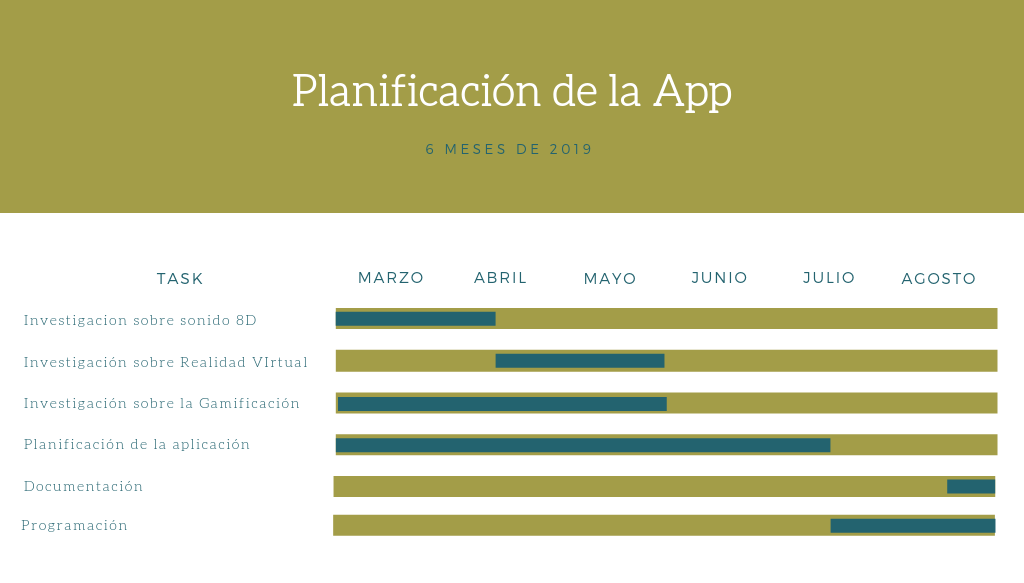
\includegraphics[width=1\textwidth]{./imagenes/diagramaGantt}
	\caption{Distribución del tiempo de desarrollo de la aplicación}
\end{figure}

\subsection{Costes e ingresos}

\quad Al no tener que pagar licencias de ningun programa utilizado, así como no necesitar comprar ningún aparato extra, la inversión monetaria en este proyecto ha sido cero.\\

\quad Por otro lado, la aplicación solo varía un poco un algoritmo ya existente, de forma que no se espera ningún tipo de beneficio por parte de esta aplicación, que solo es un campo de testeo para el algoritmo. \\

\quad Debido a que los algoritmos no se pueden patentar (al menos en España), tampoco se esperan beneficios de ningún tipo debidos a este factor.\\

\quad La intención de este proyecto era sin ánimo de lucro, por lo que al no haber tenido que invertir nada económicamente hablando ya hace que sea un balance positivo desde la perspectiva del desarrollador, quien solo ha invertido su tiempo y esfuerzo.\\ 

\newpage




